\begin{name}
	{\tenchude}{\tendethi}{LỚP TOÁN THẦY PHÁT}{\thoigian}
\end{name}
\setcounter{ex}{0}\setcounter{bt}{0}
\Opensolutionfile{ans}[ans/ans-2-TT-15-DaoSonTay-HCM-23]
\begin{ex}%[Hoàng Thanh Phương]%[2H2Y1-2]
	Trong không gian, cho tam giác $ABC$ đều cạnh $2a$. Gọi $M$ là trung điểm $BC$. Khi quay tam giác $ABC$ xung quanh trục $AM$ thì đường gấp khúc $ABC$ tạo thành một hình nón. Tính diện tích xung quanh của hình nón đó.
	\choice
	{\True $S_{\text{xq}}=2\pi a^2$}
	{$S_{\text{xq}}=4\pi a^2$}
	{$S_{\text{xq}}=6\pi a^2$}
	{$S_{\text{xq}}=8\pi a^2$}
\loigiai{Hình nón đã cho có đường sinh $\ell=2a$ và bán kính $r=BM=a$, nên diện tích xung quanh của hình nón là $S_{\text{xq}}=2\pi a^2$.}
\end{ex}
\begin{ex}%[Hoàng Thanh Phương]%[2H1Y3-2]
	Thể tích của khối chóp có đáy là tam giác đều cạnh $a$ và chiều cao $4a$ bằng
	\choice
	{$a^3\sqrt{3}$}
	{$4a^3$}
	{\True $\dfrac{a^3\sqrt{3}}{3}$}
	{$\dfrac{4}{3}a^3$}
	\loigiai{Thể tích của khối chóp đã cho là $S=\dfrac{1}{3}\cdot 4a\cdot \dfrac{a^2\sqrt{3}}{4}=\dfrac{a^3\sqrt{3}}{3}$.
}
\end{ex}
\begin{ex}%[Hoàng Thanh Phương]%[2D3Y1-1]
	Họ các nguyên hàm của hàm số $f(x)=\mathrm{e}^{2x+3}$ là
	\choice
	{$\displaystyle\int f(x)\mathrm{\,d}x=\dfrac{1}{3}\mathrm{e}^{2x+3}+C$}
	{\True $\displaystyle\int f(x)\mathrm{\,d}x=\dfrac{1}{2}\mathrm{e}^{2x+3}+C$}
	{$\displaystyle\int f(x)\mathrm{\,d}x=\mathrm{e}^{2x+3}+C$}
	{$\displaystyle\int f(x)\mathrm{\,d}x=2\mathrm{e}^{2x+3}+C$}
	\loigiai{Ta có $\displaystyle\int \mathrm{e}^{2x+3}\mathrm{\,d}x=\dfrac{1}{2}\mathrm{e}^{2x+3}+C$.
}
\end{ex}
\begin{ex}%[Hoàng Thanh Phương]%[2D2Y2-1]
	Tập xác định của hàm số $y=(x+2)^{\tfrac{3}{4}}$ là
	\choice
	{\True $(-2;+\infty)$}
	{$[-2;+\infty)$}
	{$\mathbb{R}$}
	{$(0;+\infty)$}
	\loigiai{Hàm số $y=(x+2)^{\tfrac{3}{4}}$ xác định khi và chỉ khi $x+2>0\Leftrightarrow x>-2$.}
\end{ex}
\begin{ex}%[Hoàng Thanh Phương]%[2H3Y2-2]
	Trong không gian $Oxyz$, véc-tơ $\vec{n}=(1;-1;-3)$ là một véc-tơ pháp tuyến của mặt phẳng nào sau đây?
	\choice
	{$x+y-3z-3=0$}
	{$x-y+3z-3=0$}
	{\True $x-y-3z-3=0$}
	{$z-3z-3=0$}
	\loigiai{Véc-tơ $\vec{n}=(1;-1;-3)$ là một véc-tơ pháp tuyến của mặt phẳng $x-y-3z-3=0$.}
\end{ex}
\begin{ex}%[Hoàng Thanh Phương]%[2D1Y5-1]
	\immini{Hàm số nào dưới đây có đồ thị như đường cong trong hình bên?
	\choice
	{$y=\dfrac{2x+1}{x-1}$}
	{\True $y=x^4-2x^2-1$}
	{$y=x^3-2x^2-1$}
	{$y=-x^2+2x-1$}}
	{
\begin{tikzpicture}[scale=0.8,>=stealth, font=\footnotesize, line join=round, line cap=round]
			\def\a{1} \def\b{-2} \def\c{-1} % Hệ số
			\def\xmin{-2} \def\xmax{2}
			\def\ymin{-3} \def\ymax{4}  
			\draw[->] (\xmin,0)--(\xmax,0) node [below]{$x$};
			\draw[->] (0,\ymin)--(0,\ymax) node [left]{$y$};
			\node at (0,0) [below left]{$O$};
			\clip (\xmin+0.1,\ymin+0.1) rectangle (\xmax-0.1,\ymax-0.1);
			\draw[smooth,samples=300] plot(\x,{\a*(\x)^4+\b*(\x)^2+\c});
\end{tikzpicture}}
	\loigiai{Đồ thị hàm số đã cho là dạng đồ thị hàm bậc bốn trùng phương, có hệ số bậc bốn dương nên chỉ có thể là đồ thị hàm số $y=x^4-2x^2-1$.}
\end{ex}
\begin{ex}%[Hoàng Thanh Phương]%[2H3Y1-1]
	Trong không gian $Oxyz$, cho hai véc-tơ $\vec{u}=(1;1;0)$ và $\vec{v}=(2;0;-1)$. Tính độ dài $\left|\vec{u}+2\vec{v}\right|$.
	\choice
	{$2$}
	{$2\sqrt{2}$}
	{\True $\sqrt{30}$}
	{$\sqrt{22}$}
	\loigiai{
Ta có $\vec{u}+2\vec{v}=(5;1;-2)$ nên $\left|\vec{u}+2\vec{v}\right|=\sqrt{30}$.
}
\end{ex}
\begin{ex}%[Hoàng Thanh Phương]%[2H1Y3-2]
	Cho khối lăng trụ có diện tích đáy $B=5$ và chiều cao $h=6$. Thể tích của khối lăng trụ đã cho bằng
	\choice
	{$15$}
	{$10$}
	{$180$}
	{\True $30$}
	\loigiai{Thể tích của khối lăng trụ đã cho là $V=Bh=5\cdot 6=30$.}
\end{ex}
\begin{ex}%[Hoàng Thanh Phương]%[2D2Y6-1]
	Tập nghiệm của bất phương trình $\log_3 x<2$ là
	\choice
	{\True $(0;9)$}
	{$(0;+\infty)$}
	{$(9;+\infty)$}
	{$(-\infty;9)$}
	\loigiai{Ta có $\log_3 x<2\Leftrightarrow\heva{&x>0\\&x<9}\Leftrightarrow 0<x<9$.}
\end{ex}
\begin{ex}%[Hoàng Thanh Phương]%[2D3Y2-1]
	Nếu $\displaystyle\int\limits_0^1 f(x)\mathrm{\,d}x=3$ và $\displaystyle\int\limits_0^3 f(x)\mathrm{\,d}x=-2$ thì $\displaystyle\int\limits_1^3 f(x)\mathrm{\,d}x$ bằng
	\choice
	{$-6$}
	{\True $-5$}
	{$5$}
	{$1$}
	\loigiai{Ta có $\displaystyle\int\limits_0^3 f(x)\mathrm{\,d}x=\displaystyle\int\limits_0^1 f(x)\mathrm{\,d}x+\displaystyle\int\limits_1^3 f(x)\mathrm{\,d}x\Leftrightarrow 3+\displaystyle\int\limits_1^3 f(x)\mathrm{\,d}x=-2\Leftrightarrow \displaystyle\int\limits_1^3 f(x)\mathrm{\,d}x=-5$.}
\end{ex}
\begin{ex}%[Hoàng Thanh Phương]%[1D2Y2-1]
	Với $n$ là số nguyên dương bất kỳ, $n\ge 3$, công thức nào sau đây đúng?
	\choice
	{$\mathrm{A}^3_n=\dfrac{n!}{3!(n-3)!}$}
	{\True $\mathrm{A}^3_n=\dfrac{n!}{(n-3)!}$}
	{$\mathrm{A}^3_n=\dfrac{(n-3)!}{n!}$}
	{$\mathrm{A}^3_n=\dfrac{3!(n-3)!}{n!}$}
	\loigiai{Ta có $\mathrm{A}^3_n=\dfrac{n!}{(n-3)!}$.}
\end{ex}
\begin{ex}%[Hoàng Thanh Phương]%[2D2Y5-1]
	Phương trình $\log (4x+1)=\log (2x+5)$ có nghiệm là
	\choice
	{\True $x=2$}
	{$x=1$}
	{$x=3$}
	{$x=-1$}
	\loigiai{Ta có $\log (4x+1)=\log (2x+5)\Leftrightarrow\heva{&4x+1>0\\&4x+1=2x+5}\Leftrightarrow \heva{&x>-\dfrac{1}{4}\\&x=2}\Leftrightarrow x=2$.}
\end{ex}
\begin{ex}%[Hoàng Thanh Phương]%[2H2Y2-1]
	Diện tích $S$ của mặt cầu bán kính $r$ được tính theo công thức nào dưới đây?
	\choice
	{$S=\pi r^2$}
	{\True $S=4\pi r^2$}
	{$S=2\pi r^2$}
	{$S=\dfrac{4}{3}\pi r^2$}
	\loigiai{Diện tích $S$ của mặt cầu bán kính $r$ là $S=4\pi r^2$.}
\end{ex}
\begin{ex}%[Hoàng Thanh Phương]%[1D3Y3-3]
	Cho cấp số cộng $(u_n)$ có số hạng đầu $u_1=2$ và công sai $d=5$. Giá trị của $u_4$ bằng
	\choice
	{\True $17$}
	{$250$}
	{$12$}
	{$22$}
	\loigiai{Ta có $u_4=u_1+3d=2+3\cdot 5=17$.}
\end{ex}
\begin{ex}%[Hoàng Thanh Phương]%[2D4Y1-1]
	Phần ảo của số phức $z=3-4i$ bằng
	\choice
	{\True $-4$}
	{$4$}
	{$3$}
	{$-4i$}
	\loigiai{Phần ảo của số phức $z=3-4i$ là $-4$.}
\end{ex}
\begin{ex}%[Hoàng Thanh Phương]%[2D2Y4-2]
	Đạo hàm của hàm số $y=\ln (x^2-2x+1)$ bằng
	\choice
	{$y'=\dfrac{1}{x-1}$}
	{$y'=\dfrac{1}{x^2-2x+1}$}
	{\True $y'=\dfrac{2}{x-1}$}
	{$y'=2x-2$}
	\loigiai{Ta có $\left[\ln (x^2-2x+1)\right]'=\dfrac{2x-2}{x^2-2x+1}=\dfrac{2}{x-1}$.}
\end{ex}
\begin{ex}%[Hoàng Thanh Phương]%[2D1Y2-2]
	Cho hàm số $f(x)$ có bảng biến thiên như sau
\begin{center}

\begin{tikzpicture}
			\tkzTabInit[nocadre=false,lgt=1.2,espcl=2.5,deltacl=0.6]
			{$x$ /0.6,$y'$ /0.6,$y$ /2}
			{$-\infty$,$-1$,$0$,$1$,$+\infty$}
			\tkzTabLine{,+,$0$,-,$0$,+,$0$,-,}
			\tkzTabVar{-/$-\infty$, +/$-2$,-/$-3$,+/$-2$,-/$-\infty$}
\end{tikzpicture}
\end{center}
	Giá trị cực tiểu $y_{\text{CT}}$ của hàm số đã cho là
	\choice
	{$y_{\text{CT}}=-1$}
	{$y_{\text{CT}}=0$}
	{$y_{\text{CT}}=-2$}
	{\True $y_{\text{CT}}=-3$}
	\loigiai{Dựa vào bảng biến thiên, ta có giá trị cực tiểu của hàm số là $y_{\text{CT}}=-3$.}
\end{ex}
\begin{ex}%[Hoàng Thanh Phương]%[2D1Y1-2]
	Cho hàm số $f(x)$ có bảng biến thiên như hình dưới đây
\begin{center}

\begin{tikzpicture}
			\tkzTabInit[nocadre=false,lgt=1.2,espcl=2.5,deltacl=0.6]
			{$x$ /0.6, $y'$ /0.6, $y$ /2.5}
			{$-\infty$,$-1$,$3$,$+\infty$}
			\tkzTabLine{,+,$0$,-,$0$,+,}
			\tkzTabVar{-/$-\infty$,+/$2$,-/$0$,+/$+\infty$}
\end{tikzpicture}
\end{center}
	Hàm số đã cho nghịch biến trên khoảng nào trong các khoảng dưới đây?
	\choice
	{$(-1;+\infty)$}
	{$(0;+\infty)$}
	{$(-\infty;2)$}
	{\True $(-1;3)$}
	\loigiai{Hàm số đã cho nghịch biến trên khoảng $(-1;3)$.}
\end{ex}
\begin{ex}%[Hoàng Thanh Phương]%[2D4Y1-2]
	Trên mặt phẳng tọa độ, điểm biểu diễn số phức $z=-3+2i$ có tọa độ là
	\choice
	{\True $(-3;2)$}
	{$(2;3)$}
	{$(3;2)$}
	{$(2;-3)$}
	\loigiai{Điểm biểu diễn số phức $z=-3+2i$ có tọa độ $(-3;2)$.}
\end{ex}
\begin{ex}%[Hoàng Thanh Phương]%[2D1Y2-2]
	\immini{Cho hàm số $y=ax^4+bx^2+c~(a,b\in \mathbb{R})$ có đồ thị là đường cong như hình vẽ. Giá trị cực tiểu của hàm số đã cho là
		\choice
		{$1$}
		{$0$}
		{\True $2$}
		{$-1$}}
	{
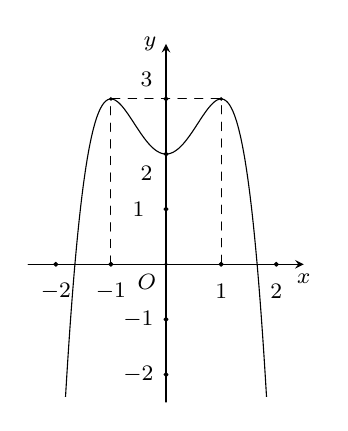
\begin{tikzpicture}[scale=0.7,>=stealth, font=\footnotesize, line join=round, line cap=round]
			\def\a{-1} \def\b{2} \def\c{2} % Hệ số
			\def\xmin{-2.5} \def\xmax{2.5}
			\def\ymin{-2.5} \def\ymax{4}  
			\draw[->] (\xmin,0)--(\xmax,0) node [below]{$x$};
			\draw[->] (0,\ymin)--(0,\ymax) node [left]{$y$};
			\node at (0,0) [below left]{$O$};
			\clip (\xmin+0.1,\ymin+0.1) rectangle (\xmax-0.1,\ymax-0.1);
			\draw[smooth,samples=300] plot(\x,{\a*(\x)^4+\b*(\x)^2+\c});
			\foreach \d/\g in{-2/-90,-1/-90,1/-90,2/-90}
			\draw[fill=black](\d,0)circle(1pt)node[shift={(\g:0.35)}]{$\d$};
			\foreach \d/\g in{-2/180,-1/180,1/180,2/-135,3/135}
			\draw[fill=black] (0,\d)circle(1pt)node[shift={(\g:0.35)}]{$\d$};
			\draw[dashed] (-1,0)--(-1,3)--(1,3)--(1,0);
			\fill[black] (0,0) circle (1pt) (-1,3) circle (1pt) (1,3) circle (1pt);
\end{tikzpicture}}
	\loigiai{Dựa vào đồ thị, giá trị cực tiểu của hàm số đã cho là $y=2$.}
\end{ex}
\begin{ex}%[Hoàng Thanh Phương]%[2D1Y4-1]
	Đường thẳng $x=2$ là tiệm cận đứng của đồ thị hàm số nào sau đây
	\choice
	{\True $y=\dfrac{x}{x-2}$}
	{$y=\dfrac{2x+1}{x+1}$}
	{$y=\dfrac{x-2}{x+2}$}
	{$y=\dfrac{-2x+3}{-x+1}$}
	\loigiai{
	Ta có $\lim\limits_{x\to 2^+}\dfrac{x}{x-2}=+\infty$ và $\lim\limits_{x\to 2^+}\dfrac{x}{x-2}=-\infty$ nên đường thẳng $x=2$ là tiệm cận đứng của đồ thị hàm số $y=\dfrac{x}{x-2}$.}
\end{ex}
\begin{ex}%[Hoàng Thanh Phương]%[2D3Y1-1]
	Họ tất cả các nguyên hàm của hàm số $f(x)=\sin x-6x^2$ là
	\choice
	{$\cos x-12x+C$}
	{$-\sin x-2x^3+C$}
	{\True $-\cos x-2x^3+C$}
	{$\sin x-12x+C$}
	\loigiai{Ta có $\displaystyle\int \left(\sin x-6x^2\right)\mathrm{\,d}x=-\cos x-2x^3+C$.}
\end{ex}
\begin{ex}%[Hoàng Thanh Phương]%[2H3Y3-3]
	Trong không gian $Oxyz$, đường thẳng $\Delta\colon \dfrac{x-1}{2}=\dfrac{y+3}{1}=\dfrac{z-2}{-3}$ đi qua điểm nào dưới đây?
	\choice
	{Điểm $P(1;3;2)$}
	{\True Điểm $N(1;-3;2)$}
	{Điểm $M(-1;3;2)$}
	{Điểm $Q(1;-3;-2)$}
	\loigiai{Đường thẳng $\Delta$ đi qua điểm $N(1;-3;2)$.}
\end{ex}
\begin{ex}%[Hoàng Thanh Phương]%[2D4Y3-2]
	Cho số phức $z$ thỏa mãn $(1-3i)z+1+7i=0$. Tổng phần thực và phần ảo của $z$ là
	\choice
	{\True $1$}
	{$3$}
	{$-3$}
	{$-6$}
	\loigiai{Ta có $z=\dfrac{-1-7i}{1-3i}=2-i$. Vậy tổng phần thực và phần ảo của $z$ là $1$.}
\end{ex}
\begin{ex}%[Hoàng Thanh Phương]%[2D4Y2-1]
	Cho hai số phức $z_1=2-3i$, $z_2=4+i$. Số phức $z=z_1-z_2$ bằng
	\choice
	{\True $-2-4i$}
	{$2-4i$}
	{$6+2i$}
	{$2-2i$}
	\loigiai{Ta có $z_1-z_2=(2-3i)-(4+i)=-2-4i$.}
\end{ex}
\begin{ex}%[Hoàng Thanh Phương]%[2D1Y5-4]
	Đồ thị hàm số $y=x^3+x^2-2x-2$ cắt trục tung tại điểm nào sau đây?
	\choice
	{$M(0;-1)$}
	{$P(-2;0)$}
	{\True $Q(0;-2)$}
	{$N(-1;0)$}
	\loigiai{Ta có $y(0)=-2$ nên đồ thị hàm số đã cho đã cho cắt trục tung tại điểm $(0;-2)$.}
\end{ex}
\begin{ex}%[Hoàng Thanh Phương]%[2H3Y1-3]
	Trong không gian $Oxyz$, cho mặt cầu $(S)\colon (x+2)^2+(y-6)^2+z^2=4$. Tâm mặt cầu $(S)$ có tọa độ là
	\choice
	{$(-1;3;0)$}
	{$(2;-6;0)$}
	{\True $(-2;6;0)$}
	{$(1;-3;0)$}
	\loigiai{Tâm của mặt cầu $(S)$ có tọa độ $(-2;6;0)$.}
\end{ex}
\begin{ex}%[Hoàng Thanh Phương]%[1D2B5-2]
	Chọn ngẫu nhiên hai số khác nhau từ $25$ số nguyên dương đầu tiên. Xác suất để chọn được hai số có tổng là một số chẵn là
	\choice
	{$\dfrac{313}{625}$}
	{\True $\dfrac{12}{25}$}
	{$\dfrac{13}{25}$}
	{$\dfrac{1}{2}$}
	\loigiai{
		Xét phép thử \lq\lq Chọn ngẫu nhiên hai số khác nhau trong $25$ số nguyên dương đầu tiên\rq\rq. \\
		Ta có $n(\Omega)=\mathrm{C}^2_{25}$. \\
		Xét biến cố $A$ \lq\lq Hai số được chọn có tổng là một số chẵn\rq\rq. \\
		Trong $25$ số nguyên dương đầu tiên có $13$ số lẻ và $12$ số chẵn.
\begin{itemize}
			\item Trường hợp $1$ : Chọn được hai số lẻ. Có $\mathrm{C}^2_{13}$ cách. 
			\item Trường hợp $2$ : Chọn được hai số chẵn. Có $\mathrm{C}^2_{12}$ cách. 
\end{itemize}
		Vậy $n(A)=\mathrm{C}^2_{13}+\mathrm{C}^2_{12}$. \\
		Xác suất của biến cố $A$ là $\mathrm{P}(A)=\dfrac{\mathrm{C}^2_{13}+\mathrm{C}^2_{12}}{\mathrm{C}^2_{25}}=\dfrac{12}{25}$.
	}
\end{ex}
\begin{ex}%[Hoàng Thanh Phương]%[2H3B2-3]
	Trong không gian $Oxyz$, cho mặt cầu $(S)$ có phương trình $x^2+y^2+z^2-2x+4y+2z-4=0$ và đi qua điểm $M(1;1;0)$. Mặt phẳng nào dưới đây tiếp xúc với mặt cầu $(S)$ tại $M$?
	\choice
	{\True $3y+z-3=0$}
	{$2x+3y+z-5=0$}
	{$3y+z-2=0$}
	{$2x+3y+z+5=0$}
	\loigiai{Mặt cầu $(S)$ có tâm $I(1;-2;-1)$ và có bán kính $R=\sqrt{10}$.\\
		Mặt phẳng tiếp xúc với mặt cầu $(S)$ tại $M$ có véc-tơ pháp tuyến là $\vec{IM}=(0;3;1)$ nên có phương trình 
		$$3(y-1)+z=0\Leftrightarrow 3y+z-3=0.$$
	}
\end{ex}
\begin{ex}%[Hoàng Thanh Phương]%[2D1B3-1]
	Trên đoạn $[0;2]$, hàm số $f(x)=x^4-2x^2+1$ đạt giá trị lớn nhất tại điểm nào sau đây?
	\choice
	{$x=0$}
	{$x=9$}
	{\True $x=2$}
	{$x=1$}
	\loigiai{Ta có $f'(x)=4x^3-4x$. \\
		$f'(x)=0\Leftrightarrow 4x^3-4x=0\Leftrightarrow\hoac{&x=-1~\text{(loại)}\\&x=0~\text{(thỏa mãn)}\\&x=1~\text{(thỏa mãn)}.}$ \\
		Ta có hàm số đã cho liên tục trên $[0;2]$ và $f(0)=1$, $f(1)=0$, $f(2)=9$. \\
		Vậy $\max\limits_{x\in [0;2]} f(x)=f(2)$, hàm số đã cho đạt giá trị lớn nhất trên đoạn $[0;2]$ tại $x=2$.
	}
\end{ex}
\begin{ex}%[Hoàng Thanh Phương]%[2D2B3-2]
	Với mọi số thực $a$ dương, $\log_2 \dfrac{a^2}{4}$ bằng
	\choice
	{$\log_2 a-2$}
	{\True $2(\log_2 a-1)$}
	{$\log_2 a-1$}
	{$2\log_2 a-1$}
	\loigiai{Với $a>0$, ta có $\log_2 \dfrac{a^2}{4}=\log_2 a^2 -\log_2 4=2\log_2 a - 2$.}
\end{ex}
\begin{ex}%[Hoàng Thanh Phương]%[1H3B5-3]
	Cho hình lăng trụ tam giác đều $ABC.A'B'C'$ có cạnh đáy bằng $2a$. Khoảng cách từ điểm $B$ tới mặt phẳng $(ACC'A')$ bằng
	\choice
	{$a\sqrt{2}$}
	{\True $a\sqrt{3}$}
	{$2\sqrt{2}a$}
	{$2a$}
	\loigiai{
		\immini{Kẻ $BH\perp AC$. Vì $ABC$ là tam giác đều nên $H$ là trung điểm $BC$. \\
			Ta có $\heva{&BH\perp AC\\&BH\perp AA'~(AA'\perp (ABC))}\Leftrightarrow BH\perp (ACC'A')$ \\
			$\Rightarrow \mathrm{d}(B,(ACC'A'))=BH$. \\
			Xét tam giác $ABC$ đều, có $BH=BC\cdot \sin C=BH\cdot \dfrac{a\sqrt{3}}{2}=a\sqrt{3}$.
		}
		{
\begin{tikzpicture}[scale=1,>=stealth, font=\footnotesize, line join=round, line cap=round]
				\path
				(0,0) coordinate (B)
				(1.5,-1.5) coordinate (A)
				(4,0) coordinate (C)
				($(A)+(0,3.2)$) coordinate (A')
				($(B)+(0,3.2)$) coordinate (B')
				($(C)+(0,3.2)$) coordinate (C')
				($(A)!0.5!(C)$) coordinate (H)
				;
				\foreach \d/\g in{B/180,A/-90,C/0,B'/180,A'/90,C'/0,H/-45}
				\draw[fill=black](\d)circle(1pt)node[shift={(\g:0.35)}]{$\d$};
				\draw (A')--(B')--(B)--(A)--(C)--(C')--(A')--(A) (B')--(C');
				\draw[dashed] (H)--(B)--(C);
				\tkzMarkRightAngles(B,H,A)
\end{tikzpicture}}	
	}
\end{ex}
\begin{ex}%[Hoàng Thanh Phương]%[2D3B2-1]
	Nếu $\displaystyle\int\limits_0^1 \left[f(x)+2x\right]\mathrm{\,d}x=2$ thì $\displaystyle\int\limits_0^1 f(x)\mathrm{\,d}x$ bằng
	\choice
	{$4$}
	{$2$}
	{$0$}
	{\True $1$}
	\loigiai{Ta có 
		$$\displaystyle\int\limits_0^1 \left[f(x)+2x\right]\mathrm{\,d}x=2\Leftrightarrow \displaystyle\int\limits_0^1 f(x)\mathrm{\,d}x=2-\displaystyle\int\limits_0^1 2x\mathrm{\,d}x=2-1=1.$$}
\end{ex}
\begin{ex}%[Hoàng Thanh Phương]%[2D2B3-2]
	Cho $\log_2 3=a$. Tính $P=\log_8 6$ theo $a$.
	\choice
	{$P=3(1+a)$}
	{\True $P=\dfrac{1}{3}(1+a)$}
	{$P=1+a$}
	{$P=2+a$}
	\loigiai{Ta có $\log_8 6=\log_8 2\cdot \log_2 6=\dfrac{1}{3}\left(1+\log_2 3\right)=\dfrac{1}{3}(1+a)$.}
\end{ex}
\begin{ex}%[Hoàng Thanh Phương]%[2D3B2-2]
	Tính tích phân $I=\displaystyle\int\limits_1^2 2x\sqrt{x^2-1}\mathrm{\,d}x$ bằng cách đặt $u=x^2-1$, mệnh đề nào dưới đây đúng?
	\choice
	{$I=\dfrac{1}{2}\displaystyle\int\limits_1^2 \sqrt{u}\mathrm{\,d}u$}
	{$I=\displaystyle\int\limits_1^2 \sqrt{u}\mathrm{\,d}u$}
	{$I=2\displaystyle\int\limits_0^3 \sqrt{u}\mathrm{\,d}u$}
	{\True $I=\displaystyle\int\limits_0^3 \sqrt{u}\mathrm{\,d}u$}
	\loigiai{
		Đặt $u=x^2-1$, ta có $\mathrm{\,d}u=2x\mathrm{\,d}x$. \\
		Đổi cận 
\begin{tabular}{c|c|c}
			$x$&$1$ &$2$ \\
			\hline
			$u$&$0$ &$3$
\end{tabular}	 \\
		Tích phân đã cho trở thành $\displaystyle\int\limits_0^3 \sqrt{u}\mathrm{\,d}u$.
	}
\end{ex}
\begin{ex}%[Hoàng Thanh Phương]%[2D1B1-1]
	Hàm số nào dưới đây đồng biến trên $\mathbb{R}$?
	\choice
	{$y=-x^3+x+1$}
	{$y=\dfrac{x-3}{x+2}$}
	{\True $y=x^3+x+1$}
	{$y=x^4+x^2$}
	\loigiai{Xét hàm số $y=x^3+x+1$. \\
	Ta có $y'=3x^2+1>0,~\forall x\in\mathbb{R}$ nên hàm số $y=x^3+x+1$ đồng biến trên $\mathbb{R}$.}
\end{ex}
\begin{ex}%[Hoàng Thanh Phương]%[1H3B4-3]
	Cho hình chóp $S.ABCD$ có đáy $ABCD$ là hình vuông cạnh $2a$, $SA$ vuông góc với đáy và $SA=a\sqrt{6}$. Góc giữa hai mặt phẳng $(SBD)$ và $(ABCD)$ bằng
	\choice
	{$45^\circ$}
	{$30^\circ$}
	{\True $60^\circ$}
	{$90^\circ$}
	\loigiai{
\immini{Ta có $\heva{&BD\perp SA\\&BD\perp AC}\Rightarrow BD\perp (SAC)\Rightarrow BD\perp SO$. \\
Có $\heva{&(SBD)\perp (ABCD)=BD\\&SO\in (SBD), SO\perp BD\\&AO\in (ABCD), AO\perp BD.}$\\
Vậy $\left((SBD),(ABCD)\right)=(SO,AO)=\widehat{SOA}$. \\
Ta có $AB=2a\Rightarrow AC=2a\sqrt{2}\Leftrightarrow AO=a\sqrt{2}$. \\
Xét tam giác $SOA$ vuông tại $A$ có $$\tan \widehat{SOA}=\dfrac{SA}{AO}=\sqrt{3}\Rightarrow \widehat{SOA}=60^\circ.$$
}
{
\begin{tikzpicture}[scale=1,>=stealth, font=\footnotesize, line join=round, line cap=round]
		\path
		(0,0) coordinate (A)
		(-1.3,-1.6) coordinate (B)
		(2.5,-1.6) coordinate (C)
		($(A)+(C)-(B)$) coordinate (D)
		($(A)+(0,3)$) coordinate (S)
		($(A)!0.5!(C)$) coordinate (O)
		;
		\draw (C)--(B)--(S)--(C)--(D)--(S);
		\draw[dashed] (O)--(S)--(A)--(C) (B)--(A)--(D)--(B);
		\foreach \d/\g in{S/90,A/180,B/180,C/0,D/0,O/-90}
		\draw[fill=black](\d)circle(1pt)node[shift={(\g:0.35)}]{$\d$};
\end{tikzpicture}}	
}
\end{ex}
\begin{ex}%[Hoàng Thanh Phương]%[2H3B2-3]
	Trong không gian $Oxyz$, cho điểm $A(4;-3;2)$. Hình chiếu vuông góc của $A$ lên các trục $Ox$, $Oy$, $Oz$ theo thứ tự là $M$, $N$, $P$. Phương trình mặt phẳng $(MNP)$ là
	\choice
	{$\dfrac{x}{4}-\dfrac{y}{3}+\dfrac{z}{2}+1=0$}
	{$4x-3y+2z-5=0$}
	{\True $3x-4y+6z-12=0$}
	{$2x-3y+4z-1=0$}
	\loigiai{
Hình chiếu của $A$ trên các trục tọa độ lần lượt là $M(4;0;0)$, $N(0;-3;0)$, $P(0;0;2)$. \\
Phương trình của mặt phẳng $(MNP)$ là 
$$\dfrac{x}{4}+\dfrac{y}{-3}+\dfrac{z}{2}=1\Leftrightarrow 3x-4y+6z-12=0.$$
}
\end{ex}
\begin{ex}%[Hoàng Thanh Phương]%[2D3K2-3]
	Cho hàm số $f(x)$ có đạo hàm liên tục trên $\mathbb{R}$. Biết $f(5)=1$ và $\displaystyle\int\limits_0^1 xf(5x)\mathrm{\,d}x=1$, khi đó $\displaystyle\int\limits_0^5 x^2f'(x)\mathrm{\,d}x$ bằng
	\choice
	{\True $-25$}
	{$23$}
	{$15$}
	{$\dfrac{123}{5}$}
	\loigiai{Xét $\displaystyle\int\limits_0^1 xf(5x)\mathrm{\,d}x=1$. \\
		Đặt $u=5x\Leftrightarrow x=\dfrac{u}{5}\Rightarrow \mathrm{\,d}x=\dfrac{1}{5}\mathrm{\,d}u$. \\
		Đổi cận 
\begin{tabular}{c|c|c}
			$x$&$0$ &$1$ \\
			\hline
			$u$&$0$ &$5$
\end{tabular} \\
		Vậy $\displaystyle\int\limits_0^1 xf(5x)\mathrm{\,d}x=1\Leftrightarrow \dfrac{1}{5} \displaystyle\int\limits_0^5 \dfrac{u}{5}f(u)\mathrm{\,d}u=1\Leftrightarrow \displaystyle\int\limits_0^5 uf(u)\mathrm{\,d}u=25\Leftrightarrow \displaystyle\int\limits_0^5 xf(x)\mathrm{\,d}x=25$. \\
		Xét $I=\displaystyle\int\limits_0^5 x^2f'(x)\mathrm{\,d}x$. \\
		Đặt $\heva{&x^2=u\\&f'(x)\mathrm{\,d}x=\mathrm{\,d}v}$, ta có $\heva{&\mathrm{\,d}u=2x\mathrm{\,d}x\\&v=f(x).}$ \\
		Khi đó $I=x^2f(x)\bigg\vert_0^5 -\displaystyle\int\limits_0^5 2xf(x)\mathrm{\,d}x=25\cdot 1- 2\cdot 25=-25$.
	}
\end{ex}
\begin{ex}%[Hoàng Thanh Phương]%[2D2K6-1]
	Có bao nhiêu số nguyên $x$ thỏa mãn $\left(2^{x^2}-4\right)\left[\log_3 (x+25)-3\right]\le 0$?
	\choice
	{$25$}
	{Vô số}
	{\True $26$}
	{$24$}
	\loigiai{Ta có $\left(2^{x^2}-4\right)\left[\log_3 (x+25)-3\right]\le 0\Leftrightarrow\hoac{&\heva{&2^{x^2}-4^x\ge 0\\&\log_3 (x+25)-3\le 0}\quad (*)\\&\heva{&2^{x^2}-4^x\le 0\\&\log_3 (x+25)-3\ge 0.}\quad (**)}$ \\
	Ta có $(*)\Leftrightarrow \heva{&x^2\ge 2x\\&x>-25\\&x+25\le 27}\Leftrightarrow \heva{&\hoac{&x\ge 2\\&x\le 0}\\&-25<x\le 2}\Leftrightarrow \hoac{&-25<x\le 0\\&x=2.}$ \\
	Ta có $(**)\Leftrightarrow \heva{&x^2\le 2x\\&x+25\ge 27}\Leftrightarrow \heva{&0\le x\le 2\\&x\ge 2}\Leftrightarrow x=2$. \\
	Vậy có $26$ số nguyên $x$ thỏa mãn yêu cầu đề bài.
}
\end{ex}
\begin{ex}%[Hoàng Thanh Phương]%[2D4K4-2]
	Trên tập hợp các số phức, xét phương trình $z^2-6z+m=0$ ($m$ là tham số thực). Gọi $m_0$ là một giá trị nguyên của $m$ để phương trình có hai nghiệm phân biệt $z_1$, $z_2$ thỏa mãn $z_1\cdot \overline{z_1}=z_2\cdot \overline{z_2}$. Trong khoảng $(0;20)$ có bao nhiêu giá trị nguyên $m_0$?
	\choice
	{$13$}
	{\True $10$}
	{$11$}
	{$12$}
	\loigiai{
		Xét phương trình $z^2-6z+m=0$. \\
		Có $\Delta'=9-m$.
\begin{itemize}
			\item TH1. Phương trình có hai nghiệm thực phân biệt $\Leftrightarrow 9-m>0\Leftrightarrow m<9$.\\
			Khi đó $\overline{z}=z$, vậy $z_1\cdot \overline{z_1}=z_2\cdot \overline{z_2}\Leftrightarrow z_1^2=z_2^2\Leftrightarrow\hoac{&z_1=z_2~\text{(loại)}\\&z_1=-z_2~\text{(thỏa mãn)}}\Rightarrow z_1+z_2=0$. \\
			Điều này mâu thuẫn vì theo định lý Vi-ét, ta có $z_1+z_2=6$.
			\item TH2. Phương trình có hai nghiệm phức liên hợp $\Leftrightarrow 9-m<0\Leftrightarrow m>9$. \\
			Ta có $z_1\cdot \overline{z_1}=z_2\cdot \overline{z_2}\Leftrightarrow z_1z_2=z_2z_1$ (luôn đúng), vậy $m\in (9;+\infty)$. \\
			Mà $m\in\mathbb{Z}$, $m<20$ nên $m\in \{10;11;\ldots;19\}$. 
\end{itemize}	
		Vậy có $10$ giá trị $m$ thỏa mãn.
	}
\end{ex}
\begin{ex}%[Hoàng Thanh Phương]%[2D1K5-3]
	\immini{Cho hàm số bậc ba $y=f(x)$ có đồ thị như hình vẽ bên. Số nghiệm thực của phương trình $\left|f\left(x^4-2x^2\right)\right|=2$ là
		\choice
		{$7$}
		{$9$}
		{$10$}
		{\True $8$}}
	{
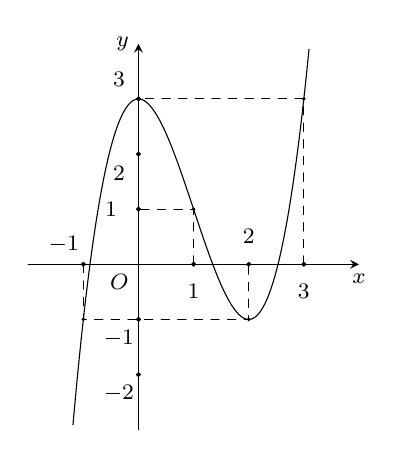
\begin{tikzpicture}[scale=0.7,>=stealth, font=\footnotesize, line join=round, line cap=round]
			\def\a{1} \def\b{-3} \def\c{0} \def\d{3} % Hệ số
			\def\xmin{-2} \def\xmax{4}
			\def\ymin{-3} \def\ymax{4} 
			\draw[->] (\xmin,0)--(\xmax,0) node [below]{$x$};
			\draw[->] (0,\ymin)--(0,\ymax) node [left]{$y$};
			\node at (0,0) [below left]{$O$};
			\clip (\xmin+0.1,\ymin+0.1) rectangle (\xmax-0.5,\ymax-0.1);
			\draw[smooth,samples=300] plot(\x,{\a*(\x)^3+\b*(\x)^2+\c*(\x)+\d});
			\foreach \d/\g in{-1/135,1/-90,2/90,3/-90}
			\draw[fill=black](\d,0)circle(1pt)node[shift={(\g:0.35)}]{$\d$};
			\foreach \d/\g in{-2/-135,-1/-135,1/180,2/-135,3/135}
			\draw[fill=black] (0,\d)circle(1pt)node[shift={(\g:0.35)}]{$\d$};
			\draw[dashed] (-1,0)--(-1,-1)--(2,-1)--(2,0) (1,0)--(1,1)--(0,1) (3,0)--(3,3)--(0,3);
			\fill[black] (-1,-1) circle (1pt)  (1,1) circle (1pt) (3,3) circle (1pt) (2,-1) circle(1pt);
\end{tikzpicture}}
	\loigiai{
		Ta có $\left|f\left(x^4-2x^2\right)\right|=2\Leftrightarrow \hoac{&f\left(x^4-2x^2\right)=-2\quad (1)\\&f\left(x^4-2x^2\right)=2.\quad (2)}$
\begin{itemize}
			\item $(1)\Leftrightarrow x^4-2x^2=a~(-2<a<-1)$.
			\item $(2)\Leftrightarrow \hoac{&x^4-2x^2=b~(-1<b<0)\\&x^4-2x^2=c ~(0<c<1)\\&x^4-2x^2=d~(2<d<3).}$
\end{itemize}
		Lập bảng biến thiên của hàm số $y=x^4-2x^2$ 
\begin{center}

\begin{tikzpicture}
				\tkzTabInit[nocadre=false,lgt=1.2,espcl=2.5,deltacl=0.6]
				{$x$ /0.6,$y'$ /0.6,$y$ /2}
				{$-\infty$,$-1$,$0$,$1$,$+\infty$}
				\tkzTabLine{,-,$0$,+,$0$,-,$0$,+,}
				\tkzTabVar{+/$+\infty$, -/$-1$,+/$0$,-/$-1$,+/$+\infty$}
\end{tikzpicture}
\end{center}
		Dựa vào bảng biến thiên ta có 
\begin{itemize}
			\item Phương trình $x^4-2x^2=a~(-2<a<-1)$ vô nghiệm.
			\item Phương trình $x^4-2x^2=b~(-1<b<0)$ có $4$ nghiệm thực phân biệt.
			\item Phương trình $x^4-2x^2=c ~(0<c<1)$ có $2$ nghiệm thực phân biệt.
			\item Phương trình $x^4-2x^2=d~(2<d<3)$ có $2$ nghiêm thực phân biệt.
\end{itemize}
		Vậy phương trình $\left|f\left(x^4-2x^2\right)\right|=2$ có $8$ nghiệm thực phân biệt.
	}
\end{ex}
\begin{ex}%[Hoàng Thanh Phương]%[2H1K3-2]
	Cho hình lăng trụ $ABC.A'B'C'$ có đáy $ABC$ là tam giác vuông tại $A$, $BC=2a$ và góc $\widehat{ABC}=60^\circ$. Biết tứ giác $BCC'B'$ là hình thoi có $B'BC$ nhọn, mặt phẳng $(BCC'B')$ vuông góc với mặt phẳng $(ABC)$, góc giữa hai mặt phẳng $(ABB'A')$ và $(ABC)$ bằng $45^\circ$. Thể tích khối lăng trụ bằng
	\choice
	{$\dfrac{a^3}{\sqrt{7}}$}
	{$\dfrac{a^3}{3\sqrt{7}}$}
	{\True $\dfrac{3a^3}{\sqrt{7}}$}
	{$\dfrac{6a^3}{\sqrt{7}}$}
	\loigiai{
		\immini{
			Xét tam giác $ABC$ vuông tại $A$ có $AB=BC\cdot \cos B=a$,\newline $AC=\sqrt{BC^2-AB^2}=a\sqrt{3}$. \\
			Kẻ $B'H\perp BC$ và $HI\parallel AC$. \\
			Vì $(BCC'B')\perp (ABC)$ nên $B'H\perp (ABC)$, suy ra $B'H\perp AB$. \\
			Mặt khác $HI\perp AB$, vậy $AB\perp (B'IH)$ nên góc giữa hai mặt phẳng $(ABB'A')$ và $(ABC)$ là $\widehat{B'IH}=45^\circ$. \\
			Vậy tam giác $B'IH$ vuông cân tại $H$. Đặt $HI=HB'=x$, ta có $BH=\sqrt{BB'^2-HB'^2}=\sqrt{4a^2-x^2}$.  \\
			Xét tam giác $IBH$ vuông tại $H$ có $$IH=BH\cdot \cos B=\sqrt{4a^2-x^2}\cdot \dfrac{\sqrt{3}}{2}.$$
		}	
		{
\begin{tikzpicture}[scale=1,>=stealth, font=\footnotesize, line join=round, line cap=round]
				\path 
				(0,0) coordinate (A)
				(1.2,-1.5) coordinate (B)
				(3.5,0) coordinate (C);
				\coordinate (H) at ($(C)!0.6!(B)$);
				\coordinate (I) at ($(A)!0.6!(B)$);
				\coordinate (B') at ($(H)+(0,4)$);
				\tkzDefPointsBy[translation = from B to B'](A,C){A'}{C'}
				\foreach \d/\g in{A/180,B/-90,C/0,A'/180,B'/90,C'/0,H/-45,I/-135}
				\draw[fill=black](\d)circle(1pt)node[shift={(\g:0.35)}]{$\d$};
				\draw (B)--(C)--(C')--(B')--(B)--(A)--(A')--(B')--(C')--(A') (I)--(B')--(H); 
				\draw[dashed] (A)--(C) (I)--(H);
				\tkzMarkRightAngles(B',H,C)
\end{tikzpicture}}
		\noindent Vậy ta có phương trình $$\sqrt{4a^2-x^2}\cdot \dfrac{\sqrt{3}}{2}=x\Rightarrow 4a^2-x^2=\dfrac{4x^2}{3}\Leftrightarrow x=\dfrac{2a\sqrt{21}}{7}.$$
		Thể tích khối lăng trụ $ABC.A'B'C'$ là $V=S_{ABC}\cdot B'H=\dfrac{1}{2}\cdot a\cdot a\sqrt{3}\cdot \dfrac{2a\sqrt{21}}{7}=\dfrac{3a^3}{\sqrt{7}}$. 
	}
\end{ex}
\begin{ex}%[Hoàng Thanh Phương]%[2D2G5-5]
	Tìm số giá trị nguyên của tham số $m$ để tồn tại các số thực $x$, $y$ thỏa mãn
	$$\mathrm{e}^{x^2+y^2-m}+\mathrm{e}^{x+y+zy-m}=x^2+y^2+x+y+xy-2m+2.$$
	\choice
	{$7$}
	{\True $9$}
	{$8$}
	{$6$}
	\loigiai{
Ta có 
\begin{eqnarray*}
	& &\mathrm{e}^{x^2+y^2-m}+\mathrm{e}^{x+y+xy-m}=x^2+y^2+x+y+xy-2m+2 \\
	&\Leftrightarrow &\mathrm{e}^{x^2+y^2-m} -(x^2+y^2-m)-1+\mathrm{e}^{x+y+xy-m}-(x+y+xy-m)-1=-2m.\quad (*)
\end{eqnarray*}	
Xét hàm $f(t)=\mathrm{e}^t-t-1$ trên $\mathbb{R}$. \\
Ta có $f'(t)=\mathrm{e}^t-1$, $f'(t)=0\Leftrightarrow t=0$. \\ 
Có $f''(t)=\mathrm{e}^t>0,~\forall t\in\mathbb{R}$ nên $t=0$ là điểm cực tiểu của hàm số $f(t)$, vậy $f(t)\ge f(0)=0~\forall t\in\mathbb{R}$. \\
Do đó $\heva{&\mathrm{e}^{x^2+y^2-m} -(x^2+y^2+m)-1\ge 0\\&\mathrm{e}^{x+y+xy-m}-(x+y+xy-m)-1\ge 0}\Rightarrow \mathrm{e}^{x^2+y^2-m}+\mathrm{e}^{x+y+zy-m}\ge x^2+y^2+x+y+xy-2m+2.$ \\
Dấu \lq\lq=\rq\rq\, xảy ra khi và chỉ khi $\heva{&x^2+y^2=m\\&x+y+xy=m.}$ \\
Đặt $S=x+y$, $P=xy$, ta có $\heva{&S^2-2P=m\\&S+P=m}\Rightarrow S^2-S-3P=0$. \\
Vì $S^2\ge 4P$ nên $S^2-S-3P=0\Rightarrow \dfrac{1}{4}S^2-S\le 0\Rightarrow 0\le S\le 4$. \\
Mặt khác, từ hệ $\heva{&S^2-2P=m\\&S+P=m}$ ta có $S^2+2S=3m$.\quad $(**)$ \\
Xét hàm số $f(S)=S^2+2S$ trên $[0;4]$. \\
Có $f'(S)=2S+2>0~\forall S\in [0;4]$ nên $f(S)$ đồng biến trên $[0;4]$. \\
Vậy $(*)$ có nghiệm khi và chỉ khi $(**)$ có nghiệm trên $[0;4]$, khi và chỉ khi $$f(0)\le 3m\le f(4)\Leftrightarrow 0\le m\le 8.$$ 
Vậy có $9$ giá trị nguyên của tham số $m$ thỏa mãn yêu cầu bài toán.
}
\end{ex}
\begin{ex}%[Hoàng Thanh Phương]%[2D4G5-1]
	Cho hai số phức $z_1$, $z_2$ thỏa mãn $|z-3-2i|=\left|\overline{z}-1\right|$, $|z_1-z_2|=2\sqrt{2}$ và số phức $w$ thỏa mãn $|w-2-4i|=1$. Giá trị nhỏ nhất của biểu thức $P=|z_2-2-3i|+|z_1-w|$ bằng
	\choice
	{$\sqrt{26}$}
	{$\sqrt{10}$}
	{\True $\sqrt{17}-1$}
	{$4$}
	\loigiai{
		\immini{
			Đặt $z=a+bi$, $a,b \in\mathbb{R}$, ta có 
\begin{eqnarray*}
				& &|z-3-2i|=\left|\overline{z}-1\right| \\
				&\Leftrightarrow &(a-3)^2+(b-2)^2=a^2+(b+1)^2 \\
				&\Leftrightarrow &a+b-3=0. 
\end{eqnarray*}	
			Vậy tập hợp các số phức $z$ là đường thẳng $d\colon x+y-3=0$. \\
			Gọi $M$ là điểm biểu diễn số phức $z_1$, $N$ là điểm biểu diễn số phức $z_2$. Ta có $|z_1-z_2|=2\sqrt{2}\Rightarrow MN=2\sqrt{2}$.}
		{
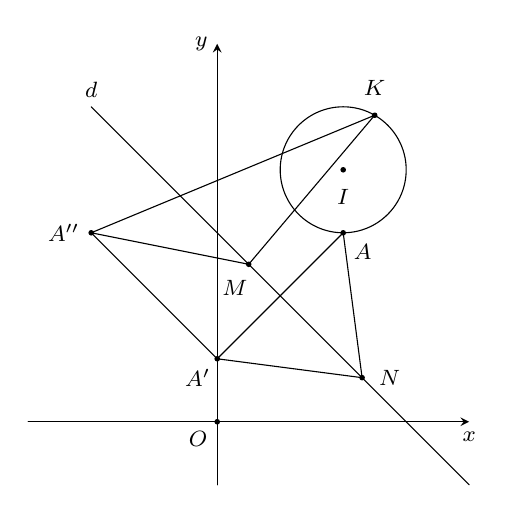
\begin{tikzpicture}[scale=0.8,>=stealth, font=\footnotesize, line join=round, line cap=round]
				\draw[->] (-3,0)--(4,0) node [below]{$x$};
				\draw[->] (0,-1)--(0,6) node [left]{$y$};
				\draw[fill=black] (0,0)node[below left]{$O$} circle (1pt);
				\path
				(2,4) coordinate (I)
				(2,3) coordinate (A)
				(0,1) coordinate (A')
				(-2,3) coordinate (A'')
				(0.5,2.5) coordinate (M)
				(2.3,0.7) coordinate (N)
				(2.5,4.866) coordinate (K)
				;
				\draw (A'')--(A')--(N)--(A)--(A') (A'')--(M)--(K)--(A'');
				\foreach \d/\g in{A/-45,I/-90,A'/-135,A''/180,M/-120,N/0,K/90}
				\draw[fill=black](\d)circle(1pt)node[shift={(\g:0.35)}]{$\d$};
				\draw (I) circle(1cm);
				\draw[smooth,samples=300,domain=4:-2] plot(\x,{-(\x)+3})node[above]{$d$};
\end{tikzpicture}}
		\noindent Gọi $K$ là điểm biểu diễn số phức $w$, ta có tập hợp điểm biểu diễn số phức $w$ là đường tròn tâm $I(2;4)$, bán kính $R=1$. \\
		Từ biểu thức đề bài ta có $P=|z_2-(2+3i)|+|z_1-w|=NA+MK$ với $A(2;3)$.\\
		Gọi $A'$ là điểm đối xứng với $A$ qua đường thẳng $d$, ta có $A'(0;1)$. Dựng $A''$ sao cho $\vec{A'A''}=\vec{NM}$, ta có $A''(-2;3)$. \\
		Ta có 
\begin{eqnarray*}
			& &P=NA+MK \\
			&=&NA'+MK \\
			&=&A''M+MK\ge A''K\ge A''I-R=\sqrt{17}-1.
\end{eqnarray*}
		Vậy giá trị nhỏ nhất của $P$ là $\sqrt{17}-1$.
	}
\end{ex}
\begin{ex}%[Hoàng Thanh Phương]%[2H3G3-7]
	Trong không gian $Oxyz$, cho hai mặt phẳng $(P)\colon x-y+z+3=0$, $(Q)\colon x+2y-2z-5=0$ và mặt cầu $(S)\colon x^2+y^2+z^2-2x+4y-6z-11=0$. Gọi $M$ là điểm di động trên $(S)$ và $N$ là điểm di động trên $(P)$ sao cho $MN$ luôn vuông góc với $(Q)$. Giá trị lớn nhất của độ dài đoạn thẳng $MN$ bằng
	\choice
	{\True $9+5\sqrt{3}$}
	{$14$}
	{$28$}
	{$3+5\sqrt{3}$}
	\loigiai{
Mặt cầu $(S)$ có tâm $I(1;-2;3)$ và bán kính $R=5$. Mặt phẳng $(P)$ có véc-tơ pháp tuyến $\vec{n}_{P}=(1;-1;1)$, mặt phẳng $(Q)$ có véc-tơ pháp tuyến $\vec{n}_{Q}=(1;2;-2)$. \\
Đường thẳng $\Delta$ đi qua hai điểm $M$ và $N$ nhận $\vec{n}_{Q}$ làm véc-tơ chỉ phương. Gọi $\varphi$ là góc tạo bởi $\Delta$ và $(P)$, $H$ là hình chiếu của $M$ trên $(P)$. \\
Ta có $\sin \varphi =\left|\cos (\vec{n}_{P},\vec{n}_{Q})\right|= \dfrac{|1\cdot 1-1\cdot 2+1\cdot (-2)|}{\sqrt{3}\cdot 3}=\dfrac{1}{\sqrt{3}}$. \\
Xét tam giác $MNH$ vuông tại $H$ có $MH=MN\cdot\sin\varphi\Rightarrow MN=\dfrac{MH}{\sin\varphi}=MH\cdot \sqrt{3}$. \\
Ta có $\mathrm{d}\left(I,(P)\right)=\dfrac{|1+2+3+3|}{\sqrt{3}}=3\sqrt{3}$. \\
Có $MH=\mathrm{d}\left(M,(P)\right)\le R+\mathrm{d}\left(I,(P)\right)=5+3\sqrt{3}$, vậy $MN=\sqrt{3}\cdot MH\le 9+5\sqrt{3}$. \\
Vậy giá trị lớn nhất của $MN$ là $9+5\sqrt{3}$.
}
\end{ex}
\begin{ex}%[Hoàng Thanh Phương]%[2H3G3-7]
	Trong không gian với hệ tọa độ $Oxyz$, từ điểm $A(1;1;0)$ ta kẻ các tiếp tuyến đến mặt cầu $(S)$ có tâm $I(-1;1;1)$, bán kính $R=1$. Gọi $M(a;b;c)$ là một trong các tiếp điểm ứng với các tiếp tuyến trên. Tìm giá trị lớn nhất của biểu thức $T=|2a-b+2c|$.
	\choice
	{$\dfrac{3+\sqrt{41}}{15}$}
	{$\dfrac{3+\sqrt{41}}{5}$}
	{$\dfrac{3+2\sqrt{41}}{15}$}
	{\True $\dfrac{3+2\sqrt{41}}{5}$}
	\loigiai{
\begin{center}
\begin{tikzpicture}[scale=0.8,>=stealth, font=\footnotesize, line join=round, line cap=round]
		\path 
		(0,0) coordinate (I)
		(-6,0) coordinate (A)
		(-0.67,1.89) coordinate (M)
		(-0.67,-1.89) coordinate (N)
		($(M)!0.5!(N)$) coordinate (E)
		;
		\draw (I) circle(2cm);
		\draw (I)--(A)--(M)--(N)--(A) (M)--(I)--(N);
		\foreach \d/\g in{I/0,M/90,N/-90,E/-135,A/180}
		\draw[fill=black](\d)circle(1pt)node[shift={(\g:0.35)}]{$\d$};
		\tkzMarkRightAngles(A,M,I A,N,I)
\end{tikzpicture}
\end{center}
Do $AM$ là tiếp tuyến của mặt cầu $(S)$ nên $AM\perp IM$, do đó tam giác $IAM$ vuông tại $M$. \\
Xét tam giác $IAM$ vuông tại $M$ có $MA=\sqrt{IA^2-R^2}=2$. \\
Vậy $M$ thuộc đường tròn giao tuyến của mặt cầu $(S)$ tâm $I$, bán kính $R=1$ và mặt cầu $(C')$ tâm $A$ bán kính $R=2$. \\
Phương trình mặt cầu $(C)$ là $(x+1)^2+(y-1)^2+(z-1)^2=1$. \\
Phương trình mặt cầu $(C')$ là $(x-1)^2+(y-1)^2+z^2=4$. \\
Phương trình mặt phẳng giao tuyến của $(C)$ và $(C')$ là
$$\heva{&(x+1)^2+(y-1)^2+(z-1)^2=1\\&(x-1)^2+(y-1)^2+z^2=4}\Leftrightarrow 2x-z+2=0.$$
Có $\vec{IA}=(2;0;-1)$ nên phương trình đường thẳng $IA$ là $\heva{&x=1+2t\\&y=1\\&z=-t.}$ \\
Gọi $E$ là tâm đường tròn giao tuyến của $(C)$ và $(C')$. Tọa độ điểm $E$ là nghiệm của hệ phương trình 
$$\heva{&x=1+2t\\&y=1\\&z=-t\\&2x-z+2=0}\Rightarrow \heva{&x=-\dfrac{3}{5}\\&y=1\\&z=\dfrac{4}{5}.}$$ \\
Xét tam giác $AMI$ vuông tại $M$ có $MI\cdot MA=ME\cdot AI\Leftrightarrow ME=\dfrac{2}{\sqrt{5}}$. \\
Vậy $M$ thuộc mặt cầu tâm $E\left(-\dfrac{3}{5};1;\dfrac{4}{5}\right)$, bán kính $r=\dfrac{2}{\sqrt{5}}$, nên tọa độ của $M$ thỏa mãn phương trình 
$$\left(x+\dfrac{3}{5}\right)^2+(b-1)^2+\left(c-\dfrac{4}{5}\right)^2=\dfrac{4}{5}.$$
Do $M\in (P)$ nên ta có $2a-c+2=0\Leftrightarrow c=2a+2.$\\
Vì $M\in (E)$ nên suy ra $\left(a+\dfrac{3}{5}\right)^2+(b-1)^2+\left(2a+\dfrac{6}{5}\right)^2=\dfrac{4}{5}\Leftrightarrow \left(\sqrt{5}a+\dfrac{3}{\sqrt{5}}\right)^2+(b-1)^2=\dfrac{4}{5}$.\\
Có $T=|2a-b+2c|=|6a-b+4|=\left|\dfrac{6}{\sqrt{5}}\left(\sqrt{5}a+\dfrac{3}{\sqrt{5}}\right)-(b-1)-\dfrac{3}{5}\right|$. \\
Áp dụng bất đẳng thức B.C.S ta có 
\begin{eqnarray*}
	& &\left|\dfrac{6}{\sqrt{5}}\left(\sqrt{5}a+\dfrac{3}{\sqrt{5}}\right)-(b-1)\right|\le \sqrt{\left[\left(\sqrt{5}a+\dfrac{3}{\sqrt{5}}\right)^2+(b-1)^2\right]\left[\left(\dfrac{6}{\sqrt{5}}\right)^2+(-1)^2\right]}=\dfrac{2\sqrt{41}}{5}\\
	&\Leftrightarrow& -\dfrac{2\sqrt{41}}{5}\le \dfrac{6}{\sqrt{5}}\left(\sqrt{5}a+\dfrac{3}{\sqrt{5}}\right)-(b-1)\le \dfrac{2\sqrt{41}}{5} \\
	&\Leftrightarrow &-\dfrac{2\sqrt{41}}{5}-\dfrac{3}{5}\le 6a-b+4\le \dfrac{2\sqrt{41}}{5}-\dfrac{3}{5}\Rightarrow T\le \dfrac{3}{5}+\dfrac{2\sqrt{41}}{5}.
\end{eqnarray*}
}
\end{ex}
\begin{ex}%[Hoàng Thanh Phương]%[2D1G5-3]
	Cho hàm số $f(x)$ liên tục trên $\mathbb{R}$ và có bảng biến thiên như sau
\begin{center}
\begin{tikzpicture}
			\tkzTabInit[nocadre=false,lgt=1.2,espcl=2.5,deltacl=0.6]
			{$x$ /0.6, $f'(x)$ /0.6, $f(x)$ /2.5}
			{$-\infty$,$-2$,$-1$,$0$,$1$,$2$,$+\infty$}
			\tkzTabLine{,+,,+,$0$,-,,-,$0$,+,,+,}
			\tkzTabVar{-/$-\infty$,R,+/$0$,R,-/$-4$,R,+/$+\infty$}
			\tkzTabIma{1}{3}{2}{$-4$}
			\tkzTabIma{3}{5}{4}{$-2$}
			\tkzTabIma{5}{7}{6}{$0$}
			\path
			($(N22)!0.5!(N23)$) coordinate (1)
			($(N42)!0.5!(N43)$) coordinate (2)
			($(N62)!0.5!(N63)$) coordinate (3);
			\draw[dashed] (L2)--(1) (L4)--(2) (L6)--(3);
\end{tikzpicture}
\end{center}
	Có bao nhiêu giá trị nguyên của tham số $m$ để phương trình $f\left[f\left(|x+1|\right)-2\right]=m$ có $10$ nghiệm phân biệt thuộc đoạn $[-3;3]$?
	\choice
	{$3$}
	{$1$}
	{\True $0$}
	{$2$}
	\loigiai{
Đặt $t=|x+1|$, vì $x\in [-3;3]$ nên $t\in [0;4]$. \\
Xét bảng biến thiên của hàm số $y=|x+1|$ trên $[-3;3]$.
\begin{center}

\begin{tikzpicture}
		\tkzTabInit[nocadre=false,lgt=1.2,espcl=2.5,deltacl=0.6]
		{$x$ /0.6,$y$ /2}
		{$-3$,$-1$,$3$}
		\tkzTabVar{+/$2$, -/$0$,+/$4$}
\end{tikzpicture}
\end{center}
Với mỗi giá trị $t\in (0;2]$ cho ta hai nghiệm $x\in [-3;3]$, còn với mỗi giá trị $t\in \{0\}\cup (2;4]$ cho ta một nghiệm $x\in [-3;3]$. \\
Phương trình đã cho trở thành $f\left(f(t)-2\right)=m$. \\
Xét hàm $g(t)=f\left(f(t)-2\right)$ trên đoạn $[0;4]$. \\
Ta có $g'(t)=f'(t)\cdot f'\left(f(t)-2\right)$. \\
$g'(t)=0\Leftrightarrow \hoac{&f'(t)=0\\&f'\left(f(t)-2\right)=0}\Leftrightarrow\hoac{&t=1 \\&t=-1~\text{(loại)}\\&f(t)-2=-1\\&f(t)-2=1}\Leftrightarrow \hoac{&t=1\\&f(t)=1\\&f(t)=3.}$  \\
Ta có 
\begin{itemize}
	\item $f(t)=1\Leftrightarrow t=t_1>2$.
	\item $f(t)=3\Leftrightarrow t=t_2>t_1>2$.
\end{itemize}
Vậy hàm số $f(t)$ có ba điểm cực trị trên đoạn $[0;4]$, suy ra phương trình $f\left(f(t)-2\right)=m$ có tối đa $4$ nghiệm $t$. Vậy phương trình đã cho có tối đa $8$ nghiệm $x$, do đó không có giá trị của tham số $m$ để phương trình đã cho có $10$ nghiệm phân biệt.
}
\end{ex}
\begin{ex}%[Hoàng Thanh Phương]%[2D3G3-1]
\immini{Cho hàm số bậc ba $y=f(x)$ có đồ thị là đường cong ở hình vẽ bên. Gọi $x_1$, $x_2$ lần lượt là hai điểm cực trị thoả mãn $x_2=x_1+2$ và $f(x_1)-3f(x_2)=0$ và đồ thị luôn đi qua $M(x_0;f(x_0))$ trong đó $x_0=x_1-1$; $g(x)$ là hàm số bậc hai có đồ thị đi qua hai điểm cực trị của đồ thị hàm số $y=f(x)$ và điểm $M$. Tính tỉ số $\dfrac{S_1}{S_2}$ ($S_1$ và $S_2$ lần lượt là diện tích hình phẳng được tạo bởi đồ thị hàm số $f(x)$, $g(x)$ như hình vẽ).
	\choice
	{$\dfrac{4}{29}$}
	{\True $\dfrac{5}{32}$}
	{$\dfrac{7}{33}$}
	{ $\dfrac{6}{35}$}
}
{
\begin{tikzpicture}[scale=0.7,>=stealth,font=\footnotesize, line join=round, line cap=round]
		\draw[->] (-.5,0)--(5.5,0)node[below] {$x$};
		\draw[->] (0,-5.5) -- (0,1)node[left] {$y$};
		\fill[pattern=north east lines, smooth] plot[domain=1:4] (\x,{(\x-2)^3-3*(\x-2)^2-1})--plot[domain=4:1] (\x,{-2*(\x-2)^2+2*(\x-2)-1});
\begin{scope}
			\clip (.8,-5.3) rectangle (5.2,.5);
			\draw[smooth,samples=200,domain=.9:5.2]
			plot(\x,{(\x-2)^3-3*(\x-2)^2-1});
			\draw[smooth,samples=200,domain=.8:4.1]
			plot(\x,{-2*(\x-2)^2+2*(\x-2)-1});
\end{scope}
		\draw[dashed] (1,0) circle (1pt)node[above] {$x_0$}  -- (1,-5) -- (0,-5) (4,0) circle (1pt)node[above] {$x_2$} -- (4,-5) -- (0,-5) circle (1pt) node[left] {$f(x_0)$} (2,0) circle (1pt)node[above] {$x_1$} -- (2,-1) circle (1pt);
		\draw[fill=black] (0,0) circle (1pt)node[above left] {$O$} (1,-5) circle (1pt) (4,-5) circle (1pt) (1,0) circle (1pt) (2,0) circle (1pt) (4,0) circle (1pt);
		\draw (1.5,-4)node{$S_1$} (2.5,-2.7)node{$S_2$};
		\node at (1,-5)[above left]{$M$};
\end{tikzpicture}}
\loigiai{
	\immini{Không mất tính tổng quát của bài toán ta có thể tịnh tiến gốc toạ độ trùng với điểm cực đại của hàm số bậc ba như hình vẽ bên. Khi đó $x_1=0$, $x_2=x_1+2=2$ và $x_0=x_1-1=-1$.\\
		Hàm số $y=f'(x)$ có hai nghiệm là $x_1=0$ và $x_2=2$ nên
		$f'(x)=3ax(x-2)=3ax^2-6ax$ với $a>0$. Suy ra $f(x)=a{x^3}-3a{x^2}+b$.\\
		Đồ thị hàm số $y=f(x)$ đi qua gốc toạ độ nên $b=0\Rightarrow f(x)=ax^3-3ax^2$.\\
		Ta có $f(-1)=f(2)=-4a$.\\
		Đồ thị parabol $(P)$ đi qua gốc toạ độ nên có dạng $(P)\colon y=mx^2+nx$.
	}
	{
\begin{tikzpicture}[scale=0.7,>=stealth,font=\footnotesize, line join=round, line cap=round]
			\draw[->] (-1.3,0)--(3.5,0)node[below] {$x$};
			\foreach \x in {-1,2}
			\draw[shift={(\x,0)}] (0pt,1pt)--(0pt,-1pt)
			node[above] {\footnotesize $\x$};
			\draw[->] (0,-4.5) -- (0,1)node[left] {$y$};
			\fill[pattern=north east lines, smooth] plot[domain=-1:2] (\x,{(\x)^3-3*(\x)^2})--plot[domain=2:-1] (\x,{-2*(\x)^2+2*(\x)});
\begin{scope}
				\clip (-1.2,-4.3) rectangle (3.1,2);
				\draw[smooth,samples=200,domain=-1.1:3.1]
				plot(\x,{(\x)^3-3*(\x)^2});
				\draw[smooth,samples=200,domain=-1.2:2.1]
				plot(\x,{-2*(\x)^2+2*(\x)});
\end{scope}
			\draw[dashed] (-1,0) -- (-1,-4) -- (0,-4) (2,0) -- (2,-4) -- (0,-4);
			\draw[fill=black] (0,0) circle (1pt)node[above left] {$O$} (-1,-4) circle (1pt) (2,-4) circle (1pt);
			\draw (-.5,-3)node{$S_1$} (.5,-1.7)node{$S_2$};
			\node at (-1,-5)[above left]{$M$};
			\fill[black] (-1,0) circle (1pt) (2,0) circle (1pt);
\end{tikzpicture}}
	\noindent Vì $(P)$ đi qua điểm $A( 2;-4a)$ và $B( -1;-4a)$ nên ta có hệ
	$$\heva{& 4m+2n=-4a \\
		& m-n=-4a}\Leftrightarrow \heva{& 4m+2n=-4a \\
		& 2m-2n=-8a}\Leftrightarrow \heva{& 6m=-12a \\
		& n=m+4a}\Leftrightarrow \heva{& m=-2a \\
		& n=2a.}$$
	Do đó parabol $(P)$ có phương trình $(P)\colon y=-2a{x^2}+2ax$.\\
	Khi đó $$S_1=\displaystyle \int\limits_{-1}^0{\left| ax^3-3ax^2-\left( -2ax^2+2ax \right) \right|\text{\, d}x}=\dfrac{5a}{12};  S_2=\displaystyle \int\limits_0^2{\left| ax^3-3ax^2-\left( -2ax^2+2ax \right) \right|\text{d}x}=\dfrac{8a}{3}.$$
	Suy ra $\dfrac{S_1}{S_2}=\dfrac{\dfrac{5a}{12}}{\dfrac{8a}{3}}=\dfrac{5}{32}$.}
\end{ex}
\begin{ex}%[Hoàng Thanh Phương]%[2H3G2-8]
	Trong không gian $Oxyz$, cho hai điểm $A(2;1;3)$, $B(6;5;5)$. Xét khối nón $(N)$ ngoại tiếp mặt cầu đường kính $AB$ có $B$ là tâm đường tròn đáy khối nón. Gọi $S$ là đỉnh của khối nón $(N)$. Khi thể tích khối nón $(N)$ nhỏ nhất thì mặt phẳng qua đỉnh $(S)$ và song song với mặt phẳng chứa đường tròn đáy của $(N)$ có phương trình $2x+by+cz+d=0$. Tính $T=b+c+d$.
	\choice
	{\True $T=12$}
	{$T=18$}
	{$T=24$}
	{$T=36$}
	\loigiai{
\immini{
Mặt cầu $(S)$ đường kính $AB$ có tâm $I(4;3;4)$ và bán kính $R=\dfrac{AB}{2}=3$. \\
Giả sử thiết diện qua trục hình nón là tam giác $SA'B'$. Gọi $r$ và $h$ lần lượt là bán kính đáy và chiều cao của hình nón ~($h>6)$. \\
Vì mặt cầu tâm $I$ nội tiếp hình nón $(N)$ nên $I$ là tâm đường tròn nội tiếp tam giác $SA'B'$.
}
{
\begin{tikzpicture}[line join=round, line cap=round, >=stealth,font=\footnotesize]%Hinh nón
		\def\a{2.5}% Bán trục lớn 
		\def\b{\a/3}% Bán trục bé
		\pgfmathsetmacro{\h}{sqrt(3)*\a}% Chiều cao
		\pgfmathsetmacro{\t}{asin(\b/\h)}
		\coordinate (M) at ({\a*cos(\t)}, {\b*sin(\t)});
		\coordinate (L) at ({-\a*cos(\t)}, {\b*sin(\t)});
		\coordinate (B) at (0,0);
		\coordinate (A') at (\a,0);
		\coordinate (B') at (-\a,0);
		\coordinate (I) at ($(S)!0.666!(B)$);
		\coordinate (A) at ($(I)!-1!(B)$);
		\coordinate (C) at ($(B')!1.5!(I)$);
		\draw[dashed] (M) arc(\t:{180-\t}:{\a} and {\b})(A')--(B');
		\path (0,\h)coordinate(S)(intersection of A'--B' and S--L)coordinate(N');
		\draw (0,\h)coordinate(S)--(L) arc({180-\t}:{360+\t}:{\a} and {\b})(M)--(0,\h);
		\pgfmathsetmacro{\s}{0.5*atan((\h-\b*sin(\t))/(\a*cos(\t)))}
		\path([rotate around ={{\s}:(N')}]A')coordinate(K)(intersection of N'--K and S--B)coordinate(H);
		\draw[dashed] let \p1 =($(B)-(H)$)in(H) circle({veclen(\x1,\y1)});
		\foreach \d/\g in{S/90,B/-90,I/180,A/135,B'/180,A'/0,C/0}
		\draw[fill=black](\d)circle(1pt)node[shift={(\g:0.35)}]{$\d$};
		\draw[dashed] (S)--(B) (I)--(C);
		\tkzMarkRightAngles(I,C,S)
\end{tikzpicture}
}	
\noindent Ta có 
\allowdisplaybreaks
\begin{eqnarray*}
	& &S_{SA'B'}=p_{SA'B'}\cdot R \\
	&\Leftrightarrow &3=\dfrac{\dfrac{1}{2}A'B'\cdot SB}{\dfrac{1}{2}\left(SB'+SA'+A'B'\right)} \\
	&\Leftrightarrow &3=\dfrac{r\cdot h}{r+l}=\dfrac{r\cdot h}{r+\sqrt{r^2+h^2}} \\
	&\Leftrightarrow & 3(r+\sqrt{r^2+h^2})=rh \\
	&\Leftrightarrow &r^2=\dfrac{9h}{h-6}.
\end{eqnarray*}
Thể tích khối nón $(N)$ là $V=\dfrac{1}{3}\pi r^2h=\dfrac{3\pi h^2}{h-6}=f(h)$. \\
Ta có $f'(h)=3\pi\cdot \dfrac{h^2-12h}{(h-6)^2}$, $f'(h)=0\Leftrightarrow \hoac{&h=0~\text{(loại)}\\&h=12~\text{(thỏa mãn)}.}$ \\
Bảng biến thiên 
\begin{center}

\begin{tikzpicture}
		\tkzTabInit[nocadre=false,lgt=1.2,espcl=2.5,deltacl=0.6]
		{$x$/0.6,$y'$/0.6,$y$/2}
		{$6$,$12$,$+\infty$}
		\tkzTabLine{,-,$0$,+,}
		\tkzTabVar{+/$+\infty$,-/$f(12)$,+/$+\infty$}
\end{tikzpicture}
\end{center}
Vậy $V$ đạt giá trị nhỏ nhất khi $h=12$, khi đó $\vec{IS}=3\vec{BI}\Rightarrow S(-2;-3;1)$.  \\
Phương trình mặt phẳng $(P)$ qua $S(-2;-3;1)$, có véc-tơ pháp tuyến $\vec{n}=\vec{BI}=(2;2;1)$ là
$$2(x+2)+2(x+3)+(z-1)=0\Leftrightarrow 2x+2y+z+9=0.$$
Vậy $b=2$, $c=1$, $d=9$ nên $b+c+d=12$.
}
\end{ex}
\Closesolutionfile{ans}
\begin{indapan}{10}
	{ans/ans-2-TT-15-DaoSonTay-HCM-23}
\end{indapan}
